\section{Proposed Method}

MOEA/D with on-line Resource Allocation by Diversity metric, MOEA/D-RAD, is a variant of MOEA/D that used a diversity metric as a way to select values for the utility function. Besides having a utility function based on a diversity metric, the algorithm is the same as MOEA/D-DE~\cite{li2009multiobjective}.

\begin{algorithm}[h]
	\caption{MOEA/D-RAD}\label{alg1}
	\begin{algorithmic}[1]

	\State Initialize the weight vectors $\lambda_i$, the neighborhood $B_i$, the utility value $u_i$ every subproblem $i=1,...,N$.
		
		\While{\textit{Termination criteria}}
		\For {1 to N}
			\If{$\textit{rand()} < u_i$}\Comment{From MOEA/D-GRA}
				\State Generate a offspring $y$ for subproblem $i$.
				\State Update the population by $y$.
			\EndIf
	\EndFor
	\State Update \textit{\textbf{u}} using a diversity metric.\Comment{Introduced here.}
		\EndWhile
	\end{algorithmic}
\end{algorithm}


The algorithm~\ref{alg1} describe MOEA/D-RAD. Except from line 4 and 7, the whole procedure in algorithm~\ref{alg1} is as in MOEA/D-DE. Likewise, all reproduction procedures are the same as in MOEA/D-DE~\cite{li2009multiobjective}. We initialize the value of the vector $u=0.5$ as in~\cite{zhou2016all}. A sensitivity analyzes need to be performed for deciding suitable values for $u$.

\subsection{Maximum Relative Diversity Loss (MRDL)} 

\begin{figure}[!t]
	\centering
	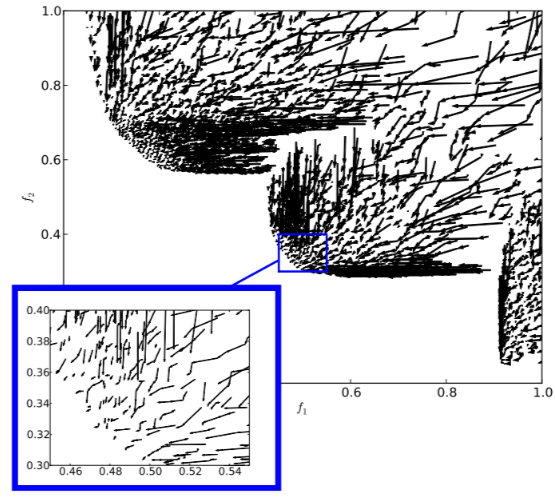
\includegraphics[width=0.47\textwidth]{img/conv_dir}
	\caption{Estimated convergence directions over 500 generations in CEC-09 UF1 benchmark test problem.Figure from~\cite{gee2015online}}
	\label{fig4}
\end{figure}

Maximum relative diversity loss (MRDL) is used to estimate the diversity loss of a solution to the whole population~\cite{gee2015online}.

 Some properties and implications of the MRDL:
\begin{itemize}
	\item If a new offspring generated is identical to any offspring solution in the convergence archive, $\Gamma^{p \rightarrow c}$  will be infinite.
	\item High values of $\Gamma^{p \rightarrow c}$ indicates the existence of similar offspring solution in the convergence archive or the offspring solution is close to the line of estimated convergence direction. 
\end{itemize}

The idea of the MRDL is to use the space movement (convergence directions) of a solution on the objective space towards the PF, as can be seen in Figure~\ref{fig4}, to calculate the diversity of the population. The further a objective vector of a solution is from the convergence direction, more it contributes for the diversity of the approximated PF.

%This is done since the convergence direction is perpendicular to the diverse direction. Here we use the definition of convergence as solutions approaching to the POF in the objective space for the first, while for diversity as the spreading and distribution of solutions along the PF~\cite{gee2015online}.


The main idea of calculating Maximum Relative Diversity Loss MRDL, $\Gamma^{p \rightarrow c}$, is to use it as a utility function as follows.

\begin{equation}
u_i = \Gamma^{p \rightarrow c}_i \text{ , with  $i=1,...,N$.}
\end{equation}

\begin{equation}
u_i = (u_i - min(u_i)) / (max(u_i) - min(u_i))
\end{equation}

\paragraph{MRDL} To calculate the MRDL, we need to compute $k$ convergence directions at every generation and then estimate the Relative Diversity Loss (RDL) for each of these $k$ convergence directions. Therefore, to estimate the diversity loss of a solution to the whole population by:
 
For every incumbent solution related to a subproblem $i$, from the whole population.

\begin{equation}
\Gamma_{i}^{p \rightarrow c} = \underset{i=1,...,k}{\max} \Gamma_{d.conv_{y}}^{p \rightarrow c}
\end{equation}


\paragraph{RDL.} RDL is a diversity measurement quantity that indicates the amount of diversity loss of an individual solution between two consecutive generations. High values of RDL imply a reduction of the solution spread and this equation may indicated the amount of diversity loss.

This quantity is given by a division between the shortest distance of a parent and offspring to the line of convergence direction.

\begin{equation}
\label{rdl}
\Gamma_{d.conv_{y}}^{p \rightarrow c} = \dfrac{ ||p \prime - proj_{d.conv_{y}}p \prime|| }{||c \prime - proj_{d.conv_{y}}c \prime||}
\end{equation}

The numerator in~\ref{rdl} is the closest distance between the parent solution ($p$) to the convergence direction $(c_r - p_r)$. While, the denominator in~\ref{rdl} is the closest distance between the offspring solution ($c$) to the convergence direction $(c_r - p_r)$. %The projections of $p\prime$ and $c\prime$ objective vectors onto the convergence direction $d.conv_{y}$ are $proj_{d.conv_{y}}p \prime$ and $proj_{d.conv_{y}}c \prime$.

with $p\prime$ and $c\prime $ given by:

\begin{equation}
\begin{split}
p\prime = p - p_r\\
c\prime = c - c_s\\
\end{split}
\end{equation}
%verify this

with $p_r$ and $c_s$ being the parent and offspring objective vectors used to calculate the convergence direction in equation~\ref{1}. That is the index $s$ is equal to the index $j$ used to calculate $conv_{y}$. The same principle is valid for the index $h$.
 
The vector projection between two vectors $a$ and $b$ that I used is defined as follows.

\begin{equation}
proj_{d.conv_{y}}p \prime = \frac {{d.conv_{y}} \cdot {p \prime}} {|{p \prime}|^2}{{p \prime}} 
\end{equation}

While the norm of $p \prime - proj_{d.conv_{y}}p \prime$ is calculated as follows.


\begin{equation}
||p \prime - proj_{d.conv_{y}}p \prime|| = sqrt(crossprod(proj_{d.conv_{y}}p \prime))
\end{equation}

The norm of $c \prime - proj_{d.conv_{y}}c \prime$ is calculated similarly.



\paragraph{Estimating convergence direction given weak-dominance relationship.}To estimate the convergence direction, $d.conv_{y}$, we need to have a offspring, $c_j$, that dominates a parent. Select a parent, $p_h$, solution that is closest to this offspring in the objective space. 

For every weakly dominated parent, one convergence direction is calculated as in the next equation.
\begin{equation}
\label{1}
	d.conv_{y} = c_j - p_h
\end{equation}

The index $j$ (for indexing offsprings, $c_j$) is selected from the set $D_c$.

\begin{equation}
\label{D}
	D_c = \{d| \exists c_d \prec p_k, k \in {1,..., N}, d \in [1,..., |C|]\}
\end{equation}

$N$ is the parent population size, $|C|$ is the size of the offspring population $C$. In equation~\ref{D}, the offspring $c_d$ must weakly dominate at least one parent solution. 

As from Zitzler et al.~\cite{zitzler2003performance} study, weak dominance ($A \succeq B$) means that any solution in B is weakly dominated by a solution in A. However, this does not rule out equality, because $A \succeq A$ for all approximation sets $A \in \Omega$.

The index $h$ (for indexing parents, $p_h$) comes from the following two equations.
\begin{equation}
h = \underset{k \in D_p }{argmin} || p_k - c_j ||
\end{equation}

\begin{equation}
\label{D_p}
D_p = \{k| \exists c_j \prec p_k, k \in {1,..., N}\}
\end{equation}

$D_p$ in equation~\ref{D_p} denotes the index set of parent solutions which are weakly dominated by $c_j$ (the $j$ index comes from equation~\ref{D}).


%\paragraph{Estimating diversity direction given the convergence direction} Diversity direction is define in~\cite{gee2015online} as the direction which is perpendicular to the converge direction.






\bibliographystyle{IEEEtran}
\bibliography{sample}


